\documentclass[11pt,paper=a4,answers]{exam}
\usepackage{graphicx,lastpage}
\usepackage{upgreek}
\usepackage{censor}
\usepackage{gensymb}
\usepackage{amsmath}
\usepackage{multicol}
\usepackage{enumitem}
\usepackage{tasks}
\usepackage{adjustbox}
\usepackage{xcolor}
\usepackage{geometry}
\geometry{margin=1in}
\usepackage{tfrupee}
\setlength{\voffset}{0.25in}
\usepackage{tabularx}
\newcolumntype{Y}{>{\centering\arraybackslash}X}
%==============================================================
% Customise Non-Essential Packages Below
% =============================================================
\usepackage[most]{tcolorbox}
\usepackage{eso-pic}
\usepackage{tikz}
\AddToShipoutPictureBG{%
\begin{tikzpicture}[remember picture,overlay]
\foreach \x in {-8,-4,0,4,8,12,16,20}
\foreach \y in {-8,-4,0,4,8,12,16,20} {
\node[opacity=0.05,rotate=45,anchor=center] at ([xshift=\x cm,yshift=\y cm]current page.center) {%
\begin{minipage}{2cm}
\centering
\includegraphics[width=2cm]{images/logo_black.png}\\
\small preppeo.com
\end{minipage}%
};
}
\end{tikzpicture}%
}
\printanswers

%==============================================================
% Customise Non-Essential Packages Above
% =============================================================
\definecolor{svgray}{rgb}{0.90, 0.90, 0.90}
\graphicspath{{images/}}

\usepackage[normalem]{ulem}
\renewcommand\ULthickness{1pt}   %%---> For changing thickness of underline
\setlength\ULdepth{3.5ex}%\maxdimen ---> For changing depth of underline
\renewcommand{\baselinestretch}{1}
\chead{
\includegraphics[scale=0.1,height=2cm ]{logo.png}
}
\pagestyle{empty}

\pagestyle{headandfoot}
\headrule
\cfoot{W: https://preppeo.com; M: +91-8130711689}

\begin{document}
%==============================================================
% Customise Question paper details below this
% =============================================================
\begin{center}
    \centering
    \renewcommand{\arraystretch}{1.5}
    \begin{tabularx}{\textwidth}{YYY}
    & \normalsize\bf{{\Large{{Quant}}}} & \\
    By Preppeo & \normalsize\bf{{sat\_lid\_005}} & SAT\\
    \normalsize{{\textbf{{Unit:}} Algebra}} & \normalsize{{\textbf{{Chapter:}} Linear equations in two variables}} & \normalsize{{\textbf{{Topic:}} Graphing Linear Equations}} \\
    \end{tabularx}
\end{center}
\par\noindent\rule{\textwidth}{1pt}
% =============================================================
% Customise Question paper details above this
% =============================================================

\begin{questions}
\pointsinrightmargin
\pointsdroppedatright
\marksnotpoints
\pointpoints{mark}{marks}
\pointformat{\boldmath\themarginpoints}
\bracketedpoints

% =============================================================
% Question Begin
% =============================================================


%Q: 1
% Category: Practice | Difficulty: Medium | Question Type: Multiple Choice
\question
The equation $4y - 3x = 12$ is graphed in the $xy$-plane. Which of the following describes the slope and the $y$-intercept of the graph?
\begin{tasks}(2)
    \task The slope is $3/4$ and the $y$-intercept is 3.
    \task The slope is $4/3$ and the $y$-intercept is 3.
    \task The slope is $3/4$ and the $y$-intercept is 12.
    \task The slope is $-3/4$ and the $y$-intercept is -3.
\end{tasks}

\begin{solution}
To find the slope and $y$-intercept of a linear equation, we must isolate $y$ to convert the equation into the slope-intercept form, $y = mx + b$. In this format, $m$ represents the slope and $b$ represents the $y$-intercept.
\\[10pt]
Starting with the given equation, $4y - 3x = 12$, we first move the $x$-term to the right side by adding $3x$ to both sides. This results in $4y = 3x + 12$. To solve for $y$ completely, we must divide every term in the entire equation by the coefficient 4.
\\[10pt]
This division gives us $y = \frac{3}{4}x + \frac{12}{4}$, which simplifies to $y = \frac{3}{4}x + 3$. By looking at the final equation, we can identify that the slope (the coefficient of $x$) is $3/4$ and the $y$-intercept (the constant term) is 3. This means the line rises 3 units for every 4 units it moves to the right.

\vspace{15pt}
Answer: \colorbox{yellow!100}{A}
\end{solution}

%Q: 2
% Category: Practice | Difficulty: Medium | Question Type: Numeric Entry
\question
A line is graphed in the $xy$-plane and passes through the origin $(0, 0)$. If the line also passes through the point $(8, 14)$, what is the slope of the line?

\begin{solution}
The slope of a line represents the steepness and direction of the line, calculated as the "rise" over the "run." Mathematically, this is the change in the $y$-coordinates divided by the change in the $x$-coordinates.
\\[10pt]
Because the line passes through the origin, we can use $(0, 0)$ as our first point and $(8, 14)$ as our second point. The change in the vertical $y$-direction is $14 - 0 = 14$. The change in the horizontal $x$-direction is $8 - 0 = 8$. 
\\[10pt]
Setting up the slope fraction, we get $14/8$. To provide a clean numeric entry, we should simplify this fraction or convert it to a decimal. Dividing 14 by 8 results in 1.75. This means that for every single unit you move to the right on the $x$-axis, the line rises by 1.75 units on the $y$-axis.

\vspace{15pt}
Answer: \colorbox{yellow!100}{1.75}
\end{solution}

%Q: 3
% Category: Practice | Difficulty: Hard | Question Type: Multiple Choice
\question
Which of the following equations represents the line shown in the graph below?
\\[10pt]
\begin{tikzpicture}[scale=0.8]
    \draw[step=1cm,gray!20,very thin] (-3,-3) grid (5,5);
    \draw[thick,->] (-3,0) -- (5,0) node[right] {$x$};
    \draw[thick,->] (0,-3) -- (0,5) node[above] {$y$};
    \draw[ultra thick, red] (-1,5) -- (5,-1);
    \filldraw (0,4) circle (2pt) node[anchor=south west] {(0,4)};
    \filldraw (4,0) circle (2pt) node[anchor=south west] {(4,0)};
\end{tikzpicture}
\begin{tasks}(2)
    \task $x + y = 4$
    \task $x - y = 4$
    \task $y = x + 4$
    \task $y = 4x$
\end{tasks}

\begin{solution}
To identify the equation from a graph, we look for key landmarks: the $y$-intercept and the $x$-intercept. In this coordinate plane, the line crosses the vertical axis at $(0, 4)$, so the $y$-intercept is 4. It crosses the horizontal axis at $(4, 0)$, so the $x$-intercept is 4.
\\[10pt]
We can find the slope by looking at the movement between these two points. Starting at $(0, 4)$ and moving to $(4, 0)$, the line goes down 4 units (a rise of -4) and moves to the right 4 units (a run of 4). The slope is $-4/4 = -1$.
\\[10pt]
Now we can write the equation in slope-intercept form as $y = -1x + 4$, or simply $y = -x + 4$. To match the multiple-choice options, we can rearrange this into standard form by adding $x$ to both sides. This gives us the final equation $x + y = 4$.

\vspace{15pt}
Answer: \colorbox{yellow!100}{A}
\end{solution}

%Q: 4
% Category: Practice | Difficulty: Medium | Question Type: Numeric Entry
\question
The graph of the linear function $f$ passes through the point $(2, 5)$ and has a $y$-intercept of $(0, 1)$. What is the slope of the graph of $f$?

\begin{solution}
To find the slope of a linear function, we need to determine how much the output ($y$) changes relative to the input ($x$) using two distinct points on the graph. The problem provides the point $(2, 5)$ and the $y$-intercept point $(0, 1)$.
\\[10pt]
The formula for the slope is $(y_2 - y_1) / (x_2 - x_1)$. Substituting our points into the formula, we have $(5 - 1)$ for the change in $y$ and $(2 - 0)$ for the change in $x$. This results in a vertical change of 4 units and a horizontal change of 2 units.
\\[10pt]
Dividing the vertical change by the horizontal change ($4 / 2$) gives us a slope of 2. This indicates that the line is increasing and specifically that for every unit you move horizontally, the graph moves up twice as much vertically.

\vspace{15pt}
Answer: \colorbox{yellow!100}{2}
\end{solution}

%Q: 5
% Category: Practice | Difficulty: Medium | Question Type: Numeric Entry
\question
What is the $x$-intercept of the line graphed by the equation $3x + 4y = 24$?

\begin{solution}
The $x$-intercept of a line is the point where the graph intersects the horizontal $x$-axis. By definition, every point located on the $x$-axis must have a vertical position (the $y$-coordinate) of exactly 0. 
\\[10pt]
To find the value of the $x$-intercept from the given equation $3x + 4y = 24$, we simply set $y$ equal to 0. This results in the simplified equation $3x + 4(0) = 24$. Since 4 multiplied by 0 is 0, the equation becomes $3x = 24$.
\\[10pt]
The final step is to isolate $x$ by dividing both sides of the equation by 3. Performing the calculation $24 / 3$ gives us 8. This tells us that the line passes through the point $(8, 0)$ on the coordinate plane, meaning the $x$-intercept is 8.

\vspace{15pt}
Answer: \colorbox{yellow!100}{8}
\end{solution}

%Q: 6
% Category: Practice | Difficulty: Medium | Question Type: Multiple Choice
\question
A line is graphed in the $xy$-plane. If the line has a negative slope and a positive $y$-intercept, which quadrant does the line NOT pass through?
\begin{tasks}(2)
    \task Quadrant I
    \task Quadrant II
    \task Quadrant III
    \task Quadrant IV
\end{tasks}

\begin{solution}

To visualize this, we look at the constraints provided. A positive $y$-intercept means the line crosses the vertical axis above the origin. This starting point is at the boundary of Quadrants I and II. 
\\[10pt]
A negative slope means the line travels "down and to the right." Moving to the right from the $y$-intercept, the line will stay in Quadrant I until it crosses the $x$-axis, after which it will enter Quadrant IV. Moving to the left from the $y$-intercept (the negative $x$ direction), the line must go "up" because the slope is negative. This path takes the line into Quadrant II.
\\[10pt]
Because the line is rising as it moves left and falling as it moves right from its positive starting point on the $y$-axis, it will occupy Quadrants I, II, and IV. It will never be able to reach Quadrant III, where both $x$ and $y$ coordinates are negative.
\vspace{15pt}
Answer: \colorbox{yellow!100}{C}
\end{solution}

%Q: 7
% Category: Practice | Difficulty: Hard | Question Type: Numeric Entry
\question
Line $k$ is perpendicular to the line $y = \frac{1}{3}x + 7$ and passes through the point $(2, 4)$. What is the $y$-intercept of line $k$?

\begin{solution}
This problem requires two steps: determining the slope of the new line and then finding its intercept. Perpendicular lines have slopes that are "negative reciprocals" of each other. This means you flip the fraction and change the sign.
\\[10pt]
The slope of the original line is $1/3$. The reciprocal is $3/1$, and changing the sign gives us a new slope of -3 for line $k$. Now we can use the slope-intercept form $y = mx + b$. We substitute the slope ($m = -3$) and the coordinates of the point $(2, 4)$ into the formula: $4 = -3(2) + b$.
\\[10pt]
Simplifying the right side gives us $4 = -6 + b$. To solve for $b$, we add 6 to both sides of the equation. This results in $10 = b$. Therefore, the $y$-intercept of line $k$ is 10, meaning it crosses the vertical axis at the point $(0, 10)$.

\vspace{15pt}
Answer: \colorbox{yellow!100}{10}
\end{solution}

%Q: 8
% Category: Practice | Difficulty: Medium | Question Type: Multiple Choice
\question
The graph of $y = f(x)$ is a line that passes through the point $(2, 1)$ and has a slope of 3. Which of the following defines the function $f$?
\begin{tasks}(2)
    \task $f(x) = 3x - 5$
    \task $f(x) = 3x + 1$
    \task $f(x) = 3x - 2$
    \task $f(x) = \frac{1}{3}x + 5$
\end{tasks}

\begin{solution}
We are given the slope $m = 3$ and a point $(2, 1)$. We can find the equation of the line by using the point-slope formula or by solving for the $y$-intercept $b$ in the equation $y = mx + b$.
\\[10pt]
Substituting the known values into the equation, we get $1 = 3(2) + b$. This simplifies to $1 = 6 + b$. To isolate $b$, we subtract 6 from both sides of the equation, which results in $b = -5$.
\\[10pt]
Now that we have both the slope and the $y$-intercept, we can write the function as $f(x) = 3x - 5$. This matches the first option provided.

\vspace{15pt}
Answer: \colorbox{yellow!100}{A}
\end{solution}

%Q: 9
% Category: Practice | Difficulty: Easy | Question Type: Numeric Entry
\question
What is the slope of any line that is parallel to the line $y = 12 - 5x$?

\begin{solution}
In coordinate geometry, one of the fundamental rules is that parallel lines always have the exact same slope. If we can identify the slope of the given line, we will have the answer for any line parallel to it.
\\[10pt]
The equation provided is $y = 12 - 5x$. Although the terms are not in the standard $y = mx + b$ order, we can identify the slope as the coefficient attached to the $x$ variable. In this case, that coefficient is -5.
\\[10pt]
Because the slope of the original line is -5, the slope of any parallel line must also be -5. This ensures that the two lines will never intersect, as they are changing at the same rate.

\vspace{15pt}
Answer: \colorbox{yellow!100}{-5}
\end{solution}

%Q: 10
% Category: Practice | Difficulty: Medium | Question Type: Multiple Choice
\question
Which of the following describes the graph of the line $x = -4$ in the $xy$-plane?
\begin{tasks}(2)
    \task A vertical line that passes through $(-4, 0)$.
    \task A horizontal line that passes through $(0, -4)$.
    \task A line with a slope of -4 that passes through the origin.
    \task A vertical line with a slope of 0.
\end{tasks}

\begin{solution}
An equation of the form $x = k$, where $k$ is a constant, represents a line where every single point has the same $x$-coordinate, regardless of the $y$-value. This results in a line that goes straight up and down.
\\[10pt]
Since the equation is $x = -4$, the line must be vertical and it must cross the horizontal axis at the value of -4. The point where it crosses the axis is $(-4, 0)$. 
\\[10pt]
Vertical lines are unique because their slope is considered "undefined" rather than zero. A slope of zero would describe a horizontal line. Therefore, the graph is a vertical line passing through $(-4, 0)$.

\vspace{15pt}
Answer: \colorbox{yellow!100}{A}
\end{solution}

%Q: 11
% Category: Practice | Difficulty: Hard | Question Type: Numeric Entry
\question
A line has an $x$-intercept of -3 and a $y$-intercept of 9. What is the slope of the line?

\begin{solution}
Intercepts provide us with two distinct points on the coordinate plane. An $x$-intercept of -3 translates to the point $(-3, 0)$, and a $y$-intercept of 9 translates to the point $(0, 9)$.
\\[10pt]
To find the slope, we use the formula for the change in $y$ divided by the change in $x$. The vertical change is $9 - 0 = 9$. The horizontal change is $0 - (-3) = 3$. 
\\[10pt]
Setting up the slope fraction, we have $9 / 3$. Simplifying this division results in a slope of 3. This positive value means that for every unit you move to the right, the line moves up by 3 units.

\vspace{15pt}
Answer: \colorbox{yellow!100}{3}
\end{solution}

%Q: 12
% Category: Practice | Difficulty: Medium | Question Type: Multiple Choice
\question
The lines $y = 2x + 4$ and $y = 2x - 5$ are graphed in the $xy$-plane. Which of the following statements is true?
\begin{tasks}(1)
    \task The lines are parallel and will never intersect.
    \task The lines are perpendicular and intersect at a right angle.
    \task The lines are the same and overlap completely.
    \task The lines intersect at the point $(0, 0)$.
\end{tasks}

\begin{solution}
To compare two linear equations, we look at their slopes ($m$) and $y$-intercepts ($b$). For the first line, $m = 2$ and $b = 4$. For the second line, $m = 2$ and $b = -5$.
\\[10pt]
Because both lines have the exact same slope but different $y$-intercepts, they are rising at the same rate but starting at different heights on the vertical axis. This is the definition of parallel lines. Parallel lines will always maintain the same distance from each other and never intersect.

\vspace{15pt}
Answer: \colorbox{yellow!100}{A}
\end{solution}

%Q: 13
% Category: Practice | Difficulty: Medium | Question Type: Numeric Entry
\question
What is the $y$-intercept of the line defined by the equation $2x - 5y = 10$?

\begin{solution}
The $y$-intercept of a line is the point where the graph crosses the vertical axis. At this location, the horizontal $x$-coordinate must be exactly 0. 
\\[10pt]
To find the $y$-value of the intercept from the equation $2x - 5y = 10$, we substitute $x$ with 0. This results in the equation $2(0) - 5y = 10$, which simplifies to $-5y = 10$.
\\[10pt]
The final step is to isolate $y$ by dividing both sides of the equation by -5. Performing the calculation $10 / -5$ results in -2. Therefore, the line crosses the $y$-axis at -2, meaning the $y$-intercept is -2.

\vspace{15pt}
Answer: \colorbox{yellow!100}{-2}
\end{solution}

%Q: 14
% Category: Practice | Difficulty: Hard | Question Type: Multiple Choice
\question
If the line $y = 3x + 2$ is reflected across the $y$-axis, what is the equation of the new line?
\begin{tasks}(2)
    \task $y = -3x + 2$
    \task $y = 3x - 2$
    \task $y = -3x - 2$
    \task $y = \frac{1}{3}x + 2$
\end{tasks}

\begin{solution}
A reflection across the $y$-axis is a geometric transformation that changes the sign of the $x$-coordinates for every point on the graph. In an algebraic equation, this is achieved by replacing every instance of $x$ with $(-x)$.
\\[10pt]
Starting with the original equation $y = 3x + 2$, we replace $x$ with $(-x)$ to get $y = 3(-x) + 2$. Simplifying this expression results in the equation $y = -3x + 2$.
\\[10pt]
Visually, the original line had a positive slope (going up and right). After the reflection, the slope becomes negative (going up and left), but it still crosses the $y$-axis at the same height of 2.

\vspace{15pt}
Answer: \colorbox{yellow!100}{A}
\end{solution}

%Q: 15
% Category: Practice | Difficulty: Medium | Question Type: Numeric Entry
\question
A line is graphed in the $xy$-plane and passes through the points $(2, 7)$ and $(4, 11)$. What is the slope of the line?

\begin{solution}
The slope of a line measures its steepness and is calculated as the ratio of the vertical change to the horizontal change between two points. 
\\[10pt]
Using the points $(2, 7)$ and $(4, 11)$, we subtract the coordinates to find these changes. The vertical change (change in $y$) is $11 - 7 = 4$. The horizontal change (change in $x$) is $4 - 2 = 2$.
\\[10pt]
The slope is the vertical change divided by the horizontal change: $4 / 2$. This simplifies to a slope of 2. This means that for every unit you move to the right, the line rises 2 units.

\vspace{15pt}
Answer: \colorbox{yellow!100}{2}
\end{solution}

%Q: 16
% Category: Practice | Difficulty: Medium | Question Type: Multiple Choice
\question
Which of the following lines is perpendicular to the $y$-axis?
\begin{tasks}(4)
    \task $y = 4$
    \task $x = 4$
    \task $y = x$
    \task $y = -x$
\end{tasks}

\begin{solution}
The $y$-axis is a vertical line. For a line to be perpendicular to it, the line must be perfectly horizontal. Horizontal lines are characterized by having a constant $y$-value and a slope of 0.
\\[10pt]
The equation for a horizontal line is always $y = k$, where $k$ is a constant. Looking at the options, $y = 4$ is the only equation that represents a horizontal line. In contrast, $x = 4$ is a vertical line (which is parallel to the $y$-axis), and $y = x$ is a diagonal line.

\vspace{15pt}
Answer: \colorbox{yellow!100}{A}
\end{solution}

%Q: 17
% Category: Practice | Difficulty: Hard | Question Type: Numeric Entry
\question
The graph of $y = 2x - 6$ forms a triangle with the $x$-axis and the $y$-axis. What is the area of this triangle?

\begin{solution}
To find the area of the triangle, we need to determine the base and the height, which are defined by the intercepts of the line on the coordinate plane.
\\[10pt]
First, find the $y$-intercept by setting $x = 0$. In $y = 2(0) - 6$, we get $y = -6$. This means the height of the triangle along the $y$-axis is 6 units (distance is always positive). Next, find the $x$-intercept by setting $y = 0$. In $0 = 2x - 6$, we add 6 to both sides and divide by 2 to get $x = 3$. This means the base of the triangle along the $x$-axis is 3 units.
\\[10pt]
The formula for the area of a triangle is $1/2 \times \text{base} \times \text{height}$. Substituting our values, we get $1/2 \times 3 \times 6 = 9$. The area of the triangle is 9 square units.

\vspace{15pt}
Answer: \colorbox{yellow!100}{9}
\end{solution}

%Q: 18
% Category: Practice | Difficulty: Medium | Question Type: Multiple Choice
\question
What is the slope of the line $x = 5$?
\begin{tasks}(4)
    \task 0
    \task 1
    \task 5
    \task Undefined
\end{tasks}

\begin{solution}
The equation $x = 5$ represents a vertical line. In a vertical line, the $x$-coordinate is the same for every point, meaning there is zero horizontal change (run).
\\[10pt]
When we use the slope formula, the denominator $(x_2 - x_1)$ will be $5 - 5 = 0$. In mathematics, division by zero is not possible and is categorized as "undefined." Therefore, all vertical lines have a slope that is undefined. If the line were horizontal, the slope would be 0.

\vspace{15pt}
Answer: \colorbox{yellow!100}{D}
\end{solution}

%Q: 19
% Category: Practice | Difficulty: Medium | Question Type: Numeric Entry
\question
The line $y = 4x + b$ passes through the point $(3, 15)$. What is the value of $b$?

\begin{solution}
To solve for the unknown constant $b$, we use the fact that any point on the line must satisfy the equation. We substitute the $x$ and $y$ coordinates of the point $(3, 15)$ into the equation.
\\[10pt]
Substituting 3 for $x$ and 15 for $y$ gives us $15 = 4(3) + b$. This simplifies to $15 = 12 + b$. To isolate $b$, we subtract 12 from both sides of the equation.
\\[10pt]
This calculation, $15 - 12$, results in 3. Therefore, the $y$-intercept of the line is 3, which means the line crosses the vertical axis at $(0, 3)$.

\vspace{15pt}
Answer: \colorbox{yellow!100}{3}
\end{solution}

%Q: 20
% Category: Practice | Difficulty: Hard | Question Type: Multiple Choice
\question
Which of the following lines is perpendicular to $y = -2x + 1$?
\begin{tasks}(2)
    \task $y = \frac{1}{2}x + 5$
    \task $y = 2x + 1$
    \task $y = -2x - 5$
    \task $y = -\frac{1}{2}x + 1$
\end{tasks}

\begin{solution}
Two lines are perpendicular if their slopes are negative reciprocals. The slope of the given line is -2.
\\[10pt]
To find the negative reciprocal of -2, we first find the reciprocal, which is -1/2, and then change the sign to positive. This gives us a required slope of $+1/2$.
\\[10pt]
Looking at the choices, the equation $y = \frac{1}{2}x + 5$ has the correct slope of $1/2$. Therefore, it is perpendicular to the original line.

\vspace{15pt}
Answer: \colorbox{yellow!100}{A}
\end{solution}

%Q: 21
% Category: Practice | Difficulty: Easy | Question Type: Numeric Entry
\question
What is the slope of the line $y = x$?

\begin{solution}
In the linear equation $y = x$, the coefficient of $x$ is not shown, but it is implicitly 1. The equation can be thought of as $y = 1x + 0$.
\\[10pt]
The slope is the coefficient of the $x$ term. Therefore, the slope of this line is 1. This means the line makes a 45-degree angle with the axes and for every unit it moves to the right, it moves up exactly one unit.

\vspace{15pt}
Answer: \colorbox{yellow!100}{1}
\end{solution}

%Q: 22
% Category: Practice | Difficulty: Medium | Question Type: Multiple Choice
\question
What is the $x$-intercept of the line $y = 2x - 8$?
\begin{tasks}(4)
    \task 4
    \task -4
    \task 8
    \task -8
\end{tasks}

\begin{solution}
The $x$-intercept is the point where $y$ is 0. Setting $y$ to 0 in the equation, we get $0 = 2x - 8$. 
\\[10pt]
Adding 8 to both sides gives $8 = 2x$. Dividing by 2, we find that $x = 4$. The line crosses the horizontal axis at 4.

\vspace{15pt}
Answer: \colorbox{yellow!100}{A}
\end{solution}

%Q: 23
% Category: Practice | Difficulty: Hard | Question Type: Numeric Entry
\question
The line $y - 3 = 2(x + 1)$ is graphed in the $xy$-plane. What is the $y$-intercept of the line?

\begin{solution}
The $y$-intercept is the point where $x = 0$. We can find this value by substituting 0 for $x$ in the point-slope equation.
\\[10pt]
Substituting $x = 0$ gives us $y - 3 = 2(0 + 1)$, which simplifies to $y - 3 = 2(1)$. This further simplifies to $y - 3 = 2$.
\\[10pt]
Adding 3 to both sides of the equation gives $y = 5$. The line intersects the vertical axis at 5.

\vspace{15pt}
Answer: \colorbox{yellow!100}{5}
\end{solution}

%Q: 24
% Category: Practice | Difficulty: Medium | Question Type: Multiple Choice
\question
A line passes through $(0, 0)$ and has a slope of -3. Which of the following is its equation?
\begin{tasks}(4)
    \task $y = -3x$
    \task $y = 3x$
    \task $x = -3y$
    \task $y = x - 3$
\end{tasks}

\begin{solution}
A line that passes through the origin has a $y$-intercept of 0. Using the slope-intercept form $y = mx + b$ with $m = -3$ and $b = 0$, the equation is $y = -3x + 0$, or $y = -3x$.
\vspace{15pt}
Answer: \colorbox{yellow!100}{A}
\end{solution}

%Q: 25
% Category: Practice | Difficulty: Medium | Question Type: Numeric Entry
\question
What is the slope of the line $4x - 4y = 12$?

\begin{solution}
To find the slope, we convert the equation to slope-intercept form ($y = mx + b$). Starting with $4x - 4y = 12$, we subtract $4x$ from both sides to get $-4y = -4x + 12$. 
\\[10pt]
Then, we divide every term by -4. This gives us $y = x - 3$. The coefficient of $x$ is 1, so the slope is 1.

\vspace{15pt}
Answer: \colorbox{yellow!100}{1}
\end{solution}

% --- SECTION 2: ADDITIONAL GRAPHING TOPICS (26-50) ---

%Q: 26
% Category: Practice | Difficulty: Medium | Question Type: Numeric Entry
\question
A line is graphed in the $xy$-plane and has the equation $y = 2x + k$. If the line passes through the point $(5, 14)$, what is the value of $k$?

\begin{solution}
To solve for $k$, we use the fact that the point $(5, 14)$ must satisfy the equation. We substitute 5 for $x$ and 14 for $y$. 
\\[10pt]
This gives us $14 = 2(5) + k$. Multiplying 2 by 5 gives 10, so the equation is $14 = 10 + k$.
\\[10pt]
Subtracting 10 from both sides of the equation reveals that $k = 4$. This value represents the $y$-intercept of the line.
\vspace{15pt}
Answer: \colorbox{yellow!100}{4}
\end{solution}

%Q: 27
% Category: Practice | Difficulty: Hard | Question Type: Multiple Choice
\question
If a line has a negative slope and a negative $y$-intercept, which quadrant does it NOT pass through?
\begin{tasks}(2)
    \task Quadrant I
    \task Quadrant II
    \task Quadrant III
    \task Quadrant IV
\end{tasks}

\begin{solution}
A negative $y$-intercept means the line crosses the $y$-axis below the origin. A negative slope means the line goes down as it moves right. Starting below the origin and moving down keeps it in Quadrant IV. Moving backwards (up and left) from the intercept takes it through Quadrant III and eventually into Quadrant II. It will never enter Quadrant I (top right) because it is starting below the $x$-axis and moving further away from it as $x$ increases.
\vspace{15pt}
Answer: \colorbox{yellow!100}{A}
\end{solution}

%Q: 28
% Category: Practice | Difficulty: Medium | Question Type: Numeric Entry
\question
What is the $x$-intercept of the line $y = -3x + 6$?

\begin{solution}
To find the $x$-intercept, we set $y = 0$. The equation becomes $0 = -3x + 6$.
\\[10pt]
Subtracting 6 from both sides gives $-6 = -3x$. Dividing both sides by -3 results in $x = 2$. The line crosses the $x$-axis at 2.
\vspace{15pt}
Answer: \colorbox{yellow!100}{2}
\end{solution}

%Q: 29
% Category: Practice | Difficulty: Medium | Question Type: Multiple Choice
\question
The line $y = 3x + 4$ is shifted down by 6 units. What is the equation of the new line?
\begin{tasks}(2)
    \task $y = 3x - 2$
    \task $y = 3x + 10$
    \task $y = -3x + 4$
    \task $y = 3x - 10$
\end{tasks}

\begin{solution}
Shifting a line vertically changes the $y$-intercept but leaves the slope the same. A shift of 6 units down means we subtract 6 from the original equation.
\\[10pt]
The new equation is $y = 3x + 4 - 6$, which simplifies to $y = 3x - 2$.
\vspace{15pt}
Answer: \colorbox{yellow!100}{A}
\end{solution}

%Q: 30
% Category: Practice | Difficulty: Medium | Question Type: Numeric Entry
\question
What is the slope of the line $2x + 5y = 20$?

\begin{solution}
To find the slope, we convert the equation to slope-intercept form. Subtract $2x$ from both sides: $5y = -2x + 20$. 
\\[10pt]
Divide every term by 5: $y = -2/5x + 4$. The slope is the coefficient of $x$, which is -0.4 or -2/5.
\vspace{15pt}
Answer: \colorbox{yellow!100}{-0.4}
\end{solution}

%Q: 31
% Category: Practice | Difficulty: Easy | Question Type: Multiple Choice
\question
Which axis is represented by the equation $y = 0$?
\begin{tasks}(2)
    \task The $x$-axis
    \task The $y$-axis
\end{tasks}

\begin{solution}
The equation $y = 0$ describes all points where the vertical position is zero. These points form the horizontal line that serves as the $x$-axis.
\vspace{15pt}
Answer: \colorbox{yellow!100}{A}
\end{solution}

%Q: 32
% Category: Practice | Difficulty: Medium | Question Type: Numeric Entry
\question
A line passes through $(0, 0)$ and $(5, 15)$. What is its slope?

\begin{solution}
Slope $= (15 - 0) / (5 - 0) = 15 / 5 = 3$.
\vspace{15pt}
Answer: \colorbox{yellow!100}{3}
\end{solution}

%Q: 33
% Category: Practice | Difficulty: Hard | Question Type: Multiple Choice
\question
Line $L$ is parallel to $x = 10$. Which point could be on line $L$?
\begin{tasks}(4)
    \task (2, 5)
    \task (10, 0)
    \task (0, 10)
    \task (10, 10)
\end{tasks}

\begin{solution}
A line parallel to $x = 10$ must also be a vertical line, meaning its equation is $x = c$ for some constant $c$. If the answer choice were $(10, 0)$, it would be the same line. If the question implies a \textit{different} parallel line, any point with the same $x$-coordinate would be on a line that overlaps. Wait, usually a parallel line in multiple choice has a different $x$. But looking at the choices, $(2, 5)$ belongs to $x=2$, which is parallel to $x=10$.
\vspace{15pt}
Answer: \colorbox{yellow!100}{A}
\end{solution}

%Q: 34
% Category: Practice | Difficulty: Hard | Question Type: Numeric Entry
\question
A line is graphed in the $xy$-plane and passes through the points $(0, 0)$ and $(h, k)$, where $h$ and $k$ are constants. If the line also passes through the point $(12, 30)$, what is the value of the ratio $\frac{k}{h}$?

\begin{solution}
The slope of a line that passes through the origin $(0, 0)$ is particularly straightforward to calculate because the change in $y$ and the change in $x$ are simply the coordinates of any other point on that line. The ratio $\frac{k}{h}$ represents the change in $y$ divided by the change in $x$ between the origin and the point $(h, k)$, which is the definition of the slope, $m$.
\\[10pt]
Since the line is straight, the slope must be constant between any two points. We are given another point on the line, $(12, 30)$. We can calculate the slope using this point and the origin: $m = \frac{30 - 0}{12 - 0}$, which simplifies to $\frac{30}{12}$. 
\\[10pt]
To find the final value, we reduce the fraction $\frac{30}{12}$ by dividing both the numerator and denominator by their greatest common factor, which is 6. This gives us $\frac{5}{2}$, or 2.5 in decimal form. Because the ratio $\frac{k}{h}$ is identical to the slope of this line, the value is 2.5.
\vspace{15pt}
Answer: \colorbox{yellow!100}{2.5}
\end{solution}

%Q: 35
% Category: Practice | Difficulty: Hard | Question Type: Multiple Choice
\question
In the $xy$-plane, the graph of line $p$ has a negative slope and a positive $y$-intercept. If line $q$ is the result of reflecting line $p$ across the $x$-axis, which of the following statements must be true about the graph of line $q$?
\begin{tasks}(2)
    \task Line $q$ has a positive slope and a negative $y$-intercept.
    \task Line $q$ has a negative slope and a negative $y$-intercept.
    \task Line $q$ has a positive slope and a positive $y$-intercept.
    \task Line $q$ has a negative slope and a positive $y$-intercept.
\end{tasks}

\begin{solution}
A reflection across the $x$-axis acts as a vertical flip of the entire coordinate plane. This transformation changes the sign of the $y$-coordinate for every point $(x, y)$ on the original line. Let's consider how this affects the slope-intercept form $y = mx + b$.
\\[10pt]
For the original line $p$, we are told the slope ($m$) is negative and the $y$-intercept ($b$) is positive. When we reflect this line across the $x$-axis, we multiply the entire equation by $-1$, changing it to $y = -(mx + b)$, which simplifies to $y = (-m)x - b$.
\\[10pt]
The new slope is the opposite of the original. Since the original slope $m$ was negative, the new slope $-m$ must be positive. Similarly, the original $y$-intercept $b$ was positive, so the new $y$-intercept $-b$ must be negative. Therefore, line $q$ will rise as it moves to the right and cross the vertical axis below the origin.
\vspace{15pt}
Answer: \colorbox{yellow!100}{A}
\end{solution}

%Q: 36
% Category: Practice | Difficulty: Medium | Question Type: Numeric Entry
\question
The line defined by the equation $x + 3y = 15$ is graphed in the $xy$-plane. If the line is shifted up by 5 units, what is the $x$-intercept of the resulting line?

\begin{solution}
To find the $x$-intercept of the new line, we should first determine the equation of the line after the vertical shift. We start by converting the original equation $x + 3y = 15$ into slope-intercept form to make the shift easier to visualize. Subtracting $x$ from both sides gives $3y = -x + 15$, and dividing by 3 gives $y = -\frac{1}{3}x + 5$.
\\[10pt]
Shifting a line "up by 5 units" means we add 5 to the $y$-intercept. The original intercept was 5, so the new intercept is $5 + 5 = 10$. The equation for our new line is $y = -\frac{1}{3}x + 10$.
\\[10pt]
The $x$-intercept occurs when $y = 0$. We substitute 0 into our new equation: $0 = -\frac{1}{3}x + 10$. Subtracting 10 from both sides gives $-10 = -\frac{1}{3}x$. Finally, we multiply both sides by $-3$ to solve for $x$, which results in $x = 30$. The new line crosses the horizontal axis at 30.
\vspace{15pt}
Answer: \colorbox{yellow!100}{30}
\end{solution}

%Q: 37
% Category: Practice | Difficulty: Hard | Question Type: Multiple Choice
\question
A line in the $xy$-plane is defined by $Ax + By = C$, where $A, B,$ and $C$ are constants such that $A > 0, B < 0,$ and $C > 0$. Which of the following best describes the slope and $y$-intercept of this line?
\begin{tasks}(2)
    \task Positive slope and positive $y$-intercept.
    \task Positive slope and negative $y$-intercept.
    \task Negative slope and positive $y$-intercept.
    \task Negative slope and negative $y$-intercept.
\end{tasks}

\begin{solution}
To analyze the slope and intercept of a line in standard form, it is helpful to rearrange it into slope-intercept form ($y = mx + b$). Starting with $Ax + By = C$, we isolate the $y$-term by subtracting $Ax$ from both sides: $By = -Ax + C$. Then, we divide every term by $B$ to get $y = (-\frac{A}{B})x + \frac{C}{B}$.
\\[10pt]
Now we evaluate the signs of the constants. We are told $A$ is positive and $B$ is negative. The ratio $\frac{A}{B}$ is therefore negative, but the slope is the negative of that ratio ($-\frac{A}{B}$), which makes the slope positive.
\\[10pt]
Next, we look at the $y$-intercept, which is $\frac{C}{B}$. We are told $C$ is positive and $B$ is negative. A positive number divided by a negative number always results in a negative value. Therefore, the $y$-intercept is negative. The line rises as it moves to the right and crosses the $y$-axis below the origin.
\vspace{15pt}
Answer: \colorbox{yellow!100}{B}
\end{solution}

%Q: 38
% Category: Practice | Difficulty: Medium | Question Type: Numeric Entry
\question
A line passes through the points $(-2, k)$ and $(4, 8)$. If the slope of the line is $0.5$, what is the value of $k$?

\begin{solution}
The slope of a line is the ratio of the vertical change to the horizontal change between two points. We can use the slope formula, $m = \frac{y_2 - y_1}{x_2 - x_1}$, and plug in the information we have to solve for the missing coordinate $k$.
\\[10pt]
Substituting the slope $m = 0.5$ and the coordinates of our two points into the formula, we get: $0.5 = \frac{8 - k}{4 - (-2)}$. This simplifies to $0.5 = \frac{8 - k}{6}$. 
\\[10pt]
To isolate the numerator, we multiply both sides of the equation by 6. Since $0.5 \times 6 = 3$, the equation becomes $3 = 8 - k$. To solve for $k$, we can subtract 8 from both sides, giving $-5 = -k$, or simply $k = 5$. This indicates the first point is $(-2, 5)$.
\vspace{15pt}
Answer: \colorbox{yellow!100}{5}
\end{solution}

%Q: 39
% Category: Practice | Difficulty: Hard | Question Type: Multiple Choice
\question
In the $xy$-plane, Line $L$ passes through the origin and is perpendicular to Line $M$, which has the equation $3x + 4y = 24$. At what point do Line $L$ and Line $M$ intersect?
\begin{tasks}(2)
    \task $(2.88, 3.84)$
    \task $(3, 3.75)$
    \task $(4, 3)$
    \task $(0, 0)$
\end{tasks}

\begin{solution}
First, we find the slope of Line $M$. Rewriting $3x + 4y = 24$ as $4y = -3x + 24$ and dividing by 4 gives $y = -0.75x + 6$. The slope of Line $M$ is $-0.75$ or $-\frac{3}{4}$. Line $L$ is perpendicular, so its slope is the negative reciprocal, which is $+\frac{4}{3}$.
\\[10pt]
Since Line $L$ passes through the origin $(0, 0)$, its equation is $y = \frac{4}{3}x$. To find the intersection, we set the two equations equal to each other or substitute $y$: $3x + 4(\frac{4}{3}x) = 24$. Multiplying by 3 to clear the fraction: $9x + 16x = 72$, which means $25x = 72$, so $x = 2.88$.
\\[10pt]
Now we find the $y$-value by plugging $x$ back into the equation for Line $L$: $y = \frac{4}{3}(2.88)$. Dividing 2.88 by 3 gives 0.96, and multiplying by 4 gives 3.84. The point of intersection is $(2.88, 3.84)$.
\vspace{15pt}
Answer: \colorbox{yellow!100}{A}
\end{solution}

%Q: 40
% Category: Practice | Difficulty: Medium | Question Type: Numeric Entry
\question
A line is graphed in the $xy$-plane and its equation is $y = 2x + 10$. If the line is reflected across the $y$-axis, what is the $x$-intercept of the resulting line?

\begin{solution}
A reflection across the $y$-axis changes the sign of the $x$-values while keeping the $y$-values the same. In the equation $y = 2x + 10$, we replace $x$ with $-x$ to find the equation of the reflected line. This results in $y = 2(-x) + 10$, or $y = -2x + 10$.
\\[10pt]
To find the $x$-intercept of this new line, we set $y = 0$ and solve for $x$. The equation becomes $0 = -2x + 10$. By adding $2x$ to both sides, we get $2x = 10$.
\\[10pt]
Finally, we divide both sides by 2, which gives us $x = 5$. This means the reflected line crosses the horizontal axis at the point $(5, 0)$. The $x$-intercept of the original line was -5, so the reflection correctly flipped it to positive 5.
\vspace{15pt}
Answer: \colorbox{yellow!100}{5}
\end{solution}

%Q: 41
% Category: Practice | Difficulty: Hard | Question Type: Multiple Choice
\question
The line $y = mx + b$ is graphed in the $xy$-plane. If the line passes through Quadrants I, II, and IV only, which of the following must be true?
\begin{tasks}(2)
    \task $m > 0$ and $b > 0$
    \task $m < 0$ and $b > 0$
    \task $m < 0$ and $b < 0$
    \task $m > 0$ and $b < 0$
\end{tasks}

\begin{solution}
To determine which quadrant a line avoids, we analyze its slope ($m$) and $y$-intercept ($b$). A line that passes through Quadrants I, II, and IV must avoid Quadrant III (where both $x$ and $y$ are negative).
\\[10pt]
If the slope $m$ were positive, the line would move "up and to the right." Moving backwards (down and to the left) from any point, it would eventually enter the negative $x$ and negative $y$ region (Quadrant III) unless it was perfectly horizontal or vertical in a way that avoids it. 
\\[10pt]
However, if the slope is negative, the line moves "down and to the right." If it starts at a positive $y$-intercept ($b > 0$), it begins in the boundary of I and II. Moving right, it stays in I and then enters IV. Moving left, it enters II. It will never cross into Quadrant III because it would need to cross the $x$-axis while $x$ is negative, which only happens if the slope is positive or if the intercept is negative. Thus, $m < 0$ and $b > 0$ is the correct condition.
\vspace{15pt}
Answer: \colorbox{yellow!100}{B}
\end{solution}

%Q: 42
% Category: Practice | Difficulty: Medium | Question Type: Numeric Entry
\question
What is the $y$-intercept of the line that is parallel to $2x + 4y = 8$ and passes through the point $(6, 10)$?

\begin{solution}
Parallel lines share the exact same slope. Our first step is to find the slope of the given line $2x + 4y = 8$. We isolate $y$ by subtracting $2x$ from both sides, giving $4y = -2x + 8$, and then dividing by 4, which results in $y = -0.5x + 2$. The slope is $-0.5$ or $-\frac{1}{2}$.
\\[10pt]
Now we use the slope-intercept form $y = mx + b$ for our new line, substituting the slope $m = -0.5$ and the point $(6, 10)$. The equation becomes $10 = -0.5(6) + b$. 
\\[10pt]
Multiplying $-0.5$ by 6 gives $-3$. The equation simplifies to $10 = -3 + b$. By adding 3 to both sides, we find that $b = 13$. The $y$-intercept of the new line is 13.
\vspace{15pt}
Answer: \colorbox{yellow!100}{13}
\end{solution}

%Q: 43
% Category: Practice | Difficulty: Hard | Question Type: Multiple Choice
\question
Which of the following lines has an $x$-intercept of 6 and is perpendicular to the line $y = 2x - 5$?
\begin{tasks}(2)
    \task $y = -0.5x + 3$
    \task $y = -2x + 12$
    \task $y = 0.5x - 3$
    \task $y = -0.5x + 6$
\end{tasks}

\begin{solution}
First, we find the required slope. The original line has a slope of 2. Perpendicular lines have negative reciprocal slopes, so the slope of our new line must be $-\frac{1}{2}$ or $-0.5$.
\\[10pt]
Next, we use the fact that the $x$-intercept is 6. This means the line must pass through the point $(6, 0)$. We can plug this point and our new slope into the $y = mx + b$ formula to solve for the $y$-intercept: $0 = -0.5(6) + b$. 
\\[10pt]
This simplifies to $0 = -3 + b$, which means $b = 3$. The equation of the line is $y = -0.5x + 3$. Checking the options, this matches the first choice.
\vspace{15pt}
Answer: \colorbox{yellow!100}{A}
\end{solution}

%Q: 44
% Category: Practice | Difficulty: Medium | Question Type: Numeric Entry
\question
What is the area of the triangle in the $xy$-plane formed by the $y$-axis, the line $y = 6$, and the line $y = 2x$?

\begin{solution}
To find the area of this triangle, we need to identify its three vertices. The first vertex is the intersection of the $y$-axis and the line $y = 6$, which is the point $(0, 6)$. The second vertex is the origin $(0, 0)$, where the line $y = 2x$ and the $y$-axis meet.
\\[10pt]
The third vertex is the intersection of the two lines $y = 6$ and $y = 2x$. We set them equal to each other: $6 = 2x$, which means $x = 3$. This intersection point is $(3, 6)$.
\\[10pt]
The triangle has a vertical side along the $y$-axis from $(0, 0)$ to $(0, 6)$, which gives it a height of 6 units. It has a horizontal distance from the $y$-axis to the point $(3, 6)$, which gives it a base of 3 units. Using the area formula $1/2 \times \text{base} \times \text{height}$, we get $1/2 \times 3 \times 6 = 9$.
\vspace{15pt}
Answer: \colorbox{yellow!100}{9}
\end{solution}

%Q: 45
% Category: Practice | Difficulty: Hard | Question Type: Multiple Choice
\question
The line $L$ contains the points $(1, k)$ and $(k, 9)$. If the slope of Line $L$ is 2, what is the value of $k$?
\begin{tasks}(4)
    \task 3.66
    \task 5
    \task 4
    \task 3.5
\end{tasks}

\begin{solution}
We use the slope formula $m = \frac{y_2 - y_1}{x_2 - x_1}$ and plug in the given slope and points. This gives us the equation $2 = \frac{9 - k}{k - 1}$.
\\[10pt]
To solve for $k$, we first multiply both sides by the denominator $(k - 1)$: $2(k - 1) = 9 - k$. Distributing the 2 gives $2k - 2 = 9 - k$.
\\[10pt]
Next, we group the $k$ terms by adding $k$ to both sides, resulting in $3k - 2 = 9$. Then, we add 2 to both sides to get $3k = 11$. Dividing by 3 gives $k = 11/3$, which is approximately 3.66.
\vspace{15pt}
Answer: \colorbox{yellow!100}{A}
\end{solution}

%Q: 46
% Category: Practice | Difficulty: Medium | Question Type: Numeric Entry
\question
What is the $y$-coordinate of the point of intersection of the lines $x + y = 10$ and $2x - y = 2$?

\begin{solution}
To find the intersection of two lines, we can solve the system of equations. Since the first equation has $+y$ and the second has $-y$, the elimination method is a very efficient choice.
\\[10pt]
Adding the two equations together $(x + y) + (2x - y) = 10 + 2$ causes the $y$ terms to cancel out, leaving $3x = 12$. Dividing by 3 gives us $x = 4$.
\\[10pt]
Now we substitute $x = 4$ back into the first equation to solve for $y$: $4 + y = 10$. Subtracting 4 from both sides reveals that $y = 6$. The two lines intersect at the point $(4, 6)$, so the $y$-coordinate of the intersection is 6.
\vspace{15pt}
Answer: \colorbox{yellow!100}{6}
\end{solution}

%Q: 47
% Category: Practice | Difficulty: Hard | Question Type: Multiple Choice
\question
Which of the following is the equation of a line that passes through $(0, 0)$ and is parallel to the line passing through $(2, 5)$ and $(4, 9)$?
\begin{tasks}(2)
    \task $y = 2x$
    \task $y = 0.5x$
    \task $y = 2x + 1$
    \task $y = -2x$
\end{tasks}

\begin{solution}
First, calculate the slope of the line passing through $(2, 5)$ and $(4, 9)$. The change in $y$ is $9 - 5 = 4$ and the change in $x$ is $4 - 2 = 2$. The slope is $4 / 2 = 2$.
\\[10pt]
Since the required line is parallel, it must have the same slope of 2. We are also told it passes through the origin $(0, 0)$, which means its $y$-intercept is 0. 
\\[10pt]
Using the $y = mx + b$ form, the equation is $y = 2x + 0$, or simply $y = 2x$.
\vspace{15pt}
Answer: \colorbox{yellow!100}{A}
\end{solution}

%Q: 48
% Category: Practice | Difficulty: Medium | Question Type: Numeric Entry
\question
If the line $y = 3x - 12$ is graphed in the $xy$-plane, what is the distance between the $x$-intercept and the $y$-intercept?

\begin{solution}
First, we find the coordinates of the two intercepts. The $y$-intercept is found by setting $x = 0$, which gives $y = -12$. This point is $(0, -12)$. The $x$-intercept is found by setting $y = 0$: $0 = 3x - 12$, which gives $12 = 3x$, so $x = 4$. This point is $(4, 0)$.
\\[10pt]
We now have the two points $(4, 0)$ and $(0, -12)$. We can use the distance formula or recognize that these points form the legs of a right triangle with the origin. The lengths of the legs are 4 and 12.
\\[10pt]
Using the Pythagorean theorem $a^2 + b^2 = c^2$, we calculate $4^2 + 12^2 = c^2$, which is $16 + 144 = 160$. The distance is the square root of 160. While $\sqrt{160}$ is the exact distance, for a numeric entry, we would provide the decimal equivalent, which is approximately 12.65.
\vspace{15pt}
Answer: \colorbox{yellow!100}{12.65}
\end{solution}

%Q: 49
% Category: Practice | Difficulty: Medium | Question Type: Multiple Choice
\question
What is the slope of a line that is perpendicular to the line passing through $(-2, 3)$ and $(4, 5)$?
\begin{tasks}(4)
    \task -3
    \task 3
    \task -1/3
    \task 1/3
\end{tasks}

\begin{solution}
First, find the slope of the line through $(-2, 3)$ and $(4, 5)$. The change in $y$ is $5 - 3 = 2$ and the change in $x$ is $4 - (-2) = 6$. The slope is $2 / 6$, which simplifies to $1/3$.
\\[10pt]
A perpendicular line must have a slope that is the negative reciprocal of $1/3$. We flip the fraction to get 3 and change the sign to negative, resulting in a slope of -3.
\vspace{15pt}
Answer: \colorbox{yellow!100}{A}
\end{solution}

%Q: 50
% Category: Practice | Difficulty: Hard | Question Type: Numeric Entry
\question
In the $xy$-plane, the line $y = mx + b$ is the reflection of the line $y = 2x + 4$ across the $x$-axis. What is the value of $m + b$?

\begin{solution}
A reflection across the $x$-axis flips the line vertically by changing the sign of all $y$-values. This is done by multiplying the entire right side of the original equation by $-1$.
\\[10pt]
Starting with $y = 2x + 4$, the reflected line has the equation $y = -(2x + 4)$, which distributes to $y = -2x - 4$.
\\[10pt]
From this new equation, we can see that the slope $m$ is -2 and the $y$-intercept $b$ is -4. The question asks for the sum $m + b$. Adding them together, $-2 + (-4)$, gives us a final result of -6.
\vspace{15pt}
Answer: \colorbox{yellow!100}{-6}
\end{solution}



% =============================================================
% Question End
% =============================================================

\end{questions}
\begin{center}
\rule{.5\textwidth}{1pt}
\end{center}
\end{document}
